%!TEX program = xelatex

\begin{titlepage}
    % Enforce precise, elegant margins for an image-based report cover
    \newgeometry{top=2.2cm,bottom=2.2cm,left=2.5cm,right=2.5cm}
    
    % Use the same serif report font as the main body for a dissertation-style cover.
    \normalfont\rmfamily
    
    % --- BLUE BAR AT THE VERY TOP ---
    \noindent
    {\color{ImperialBlue}\hrule height 4pt} % Thick corporate brand bar
    \vspace{0.2cm} % Tightens the gap between the bar and the top of the headers

    % --- BRANDING HEADER BLOCK (ASYMMETRICAL LAYOUT) ---
    \noindent
    \begin{minipage}[t]{0.55\textwidth}
        \flushleft\vspace{-4pt}
        % Top-left university logo kept exactly the same size
        
\includegraphics[height=0.65cm]{Figures/Imperial_College_London_new_logo (1).png} 
        
        \vspace{0.25cm} % Tight spacing directly beneath the logo
        {\small\textcolor{Woodsmoke}{MEng Design Engineering}\par}
        \vspace{0.05cm}
        {\small\textcolor{ImperialBlue}{\textbf{Master’s Project Report}}\par}
    \end{minipage}%
    \begin{minipage}[t]{0.45\textwidth}
        \flushright\vspace{-4pt}
        % Top-right logo scaled up larger as requested
        
\includegraphics[height=2.3cm]{Figures/dyson-school-square-transparent.png}
    \end{minipage}

    \vspace{1.2cm} % Adjusted whitespace to compensate for the text shifting up

    % --- HERO COVER IMAGE ---
    \noindent
    \begin{minipage}{\textwidth}
        \centering
        % Replaces fixed height with a dynamic width matching your layout boundaries
        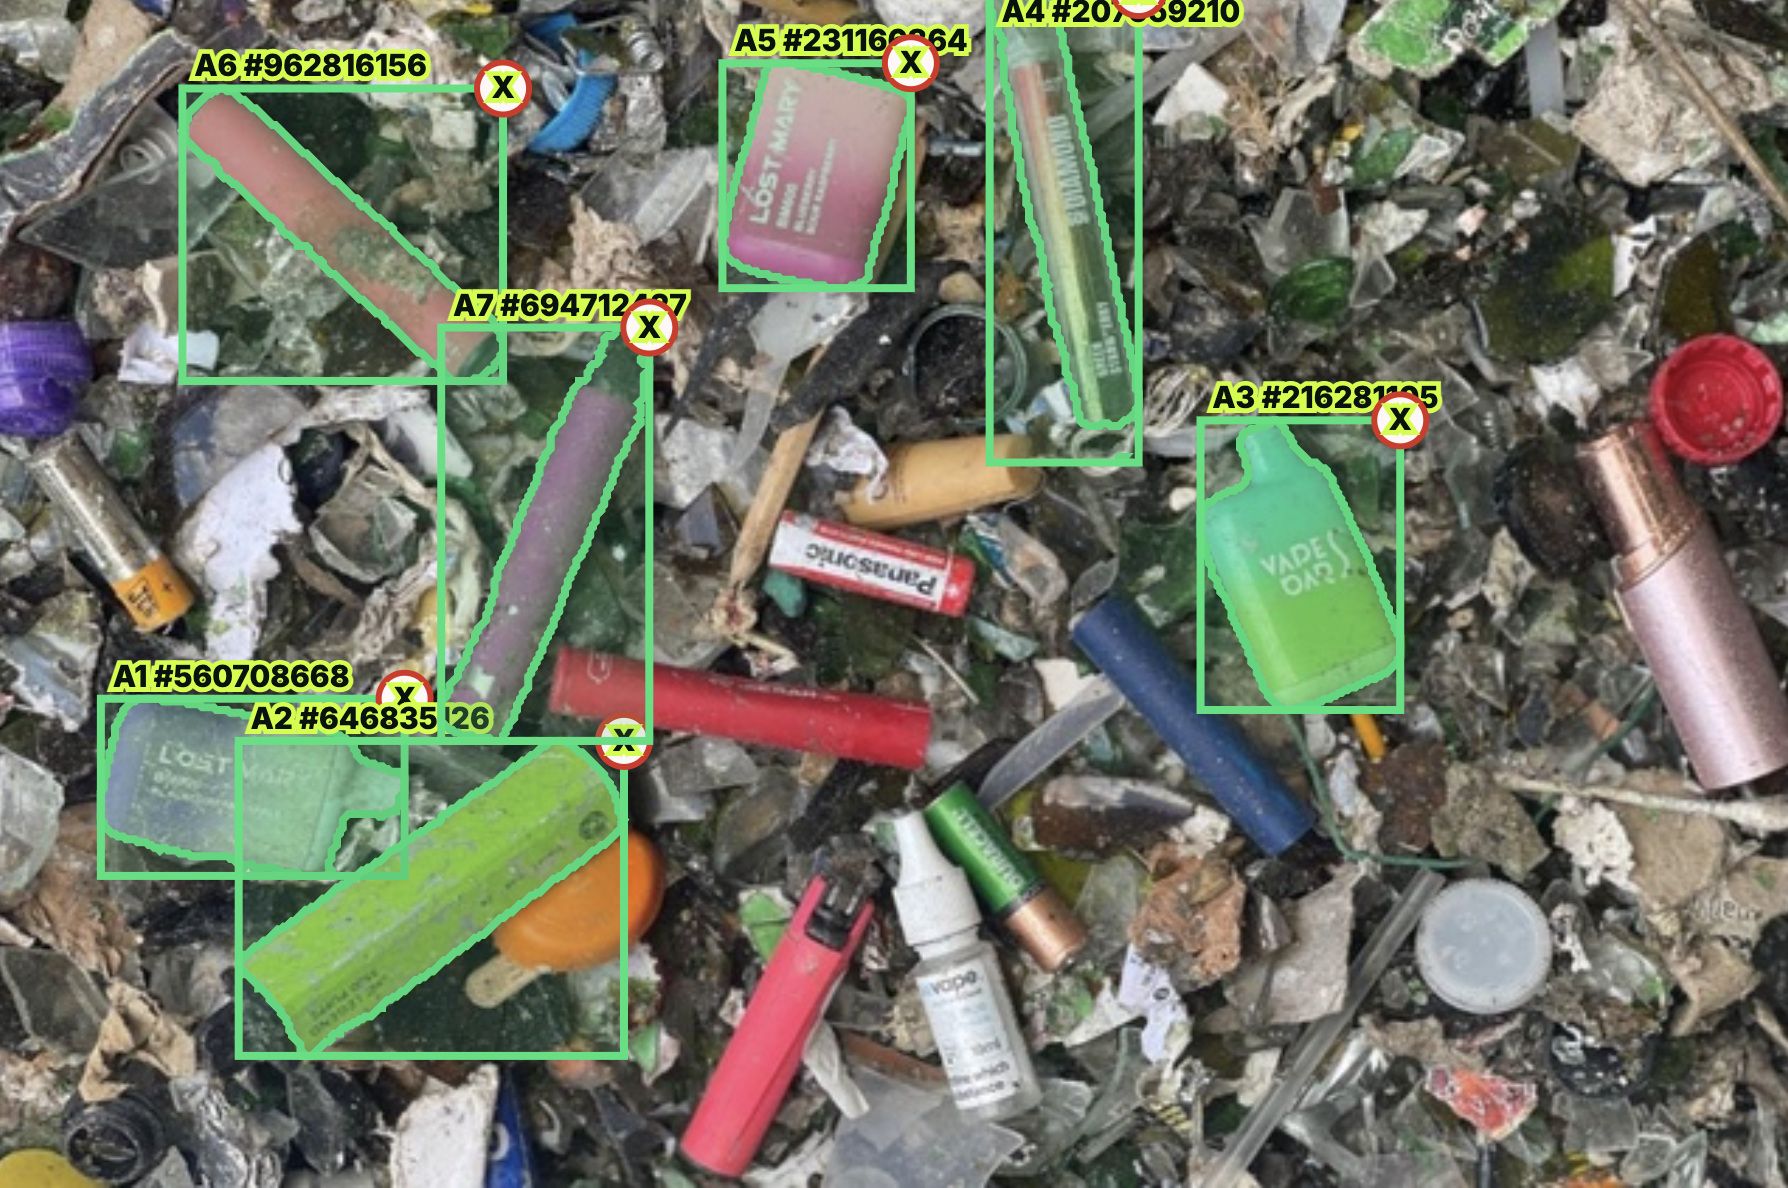
\includegraphics[width=1\linewidth, keepaspectratio]{vape_cover.png}
    \end{minipage}

    \vspace{1.5cm} % Generous white space below the image

    % --- REPORT TITLES ---
    \begin{center}
        \nopagebreak
        {\small\bfseries\textcolor{ImperialBlue}{UAVAPE PROJECT}\par}
        \vspace{0.35cm}
        {\fontsize{28pt}{33pt}\selectfont\bfseries\textcolor{Woodsmoke}{Detecting Hazardous Vape Micro-WEEE in UAV-Oriented Urban Imagery}\par}
        \par
        \vspace{0.55cm}
        {\large\textcolor{Woodsmoke}{Dataset construction, YOLO detector benchmarking and cleanup workflow prototyping for UK urban environments}\par}
    \end{center}

    \vfill

    % --- METADATA CONFIGURATION PANEL (SPLIT LEFT & RIGHT) ---
    \noindent
    \begin{minipage}[t]{0.5\textwidth}
        \flushleft
        \fontsize{10.5pt}{15pt}\selectfont
        \renewcommand{\arraystretch}{1.3}
        \begin{tabular}{ll}
            \textbf{\textcolor{ImperialBlue}{Author:}} & Zain Ahmad \\
            \textbf{\textcolor{ImperialBlue}{Supervisor:}} & Kamyar Hazeri \\
        \end{tabular}
    \end{minipage}%
    \begin{minipage}[t]{0.5\textwidth}
        \flushright
        \fontsize{10.5pt}{15pt}\selectfont
        \renewcommand{\arraystretch}{1.3}
        \begin{tabular}{rl}
            \textbf{\textcolor{ImperialBlue}{CID:}} & 02014469 \\
            \textbf{\textcolor{ImperialBlue}{Academic Year:}} & 2025--26 \\
        \end{tabular}
    \end{minipage}

    \vspace{0.4cm} % Elegant breathing room between metadata panel and bottom bar

    % --- BLUE BAR AT THE VERY BOTTOM ---
    \noindent
    {\color{ImperialBlue}\hrule height 4pt} % Thick corporate brand bar mirrored
    
    \restoregeometry
\end{titlepage}
